\chapter{CPlan}\label{CPlan}
CPlan is a tool written by the Department of Architecture of the ETH-Zurich. The goal of this application is to generate/grow street networks dynamically and extend these networks with buildings. 
\section{Improvements}
\begin{itemize}
    \item Some calls to the methods IEnumerable.ToArray() and IEnumerable.ToList() were removed. This method creates a new array / list and stores every item of the IEnumerable in this new collection. As a result the application had an extremely large footprint. To further reduce this overhead some methods were changed to take IEnumerable parameters instead of arrays.
    \item Certain graph and geometry extension methods were fixed. It would be good practice to create unit tests for such methods.
    \item matrix2D not clockwise? (TODO)
    \item Geometry2D not correct line intersection! (TODO)
\end{itemize}

\section{Genetic algorithms}
The ETH-Zurich already has genetic optimizations algorithms based on trees. Unfortunately they don't have a working solution to produce a tree from the existing graph. The new created tree generation produces a relative tree with absolute angles.

\pagebreak
\section{Normalising Street Networks}
While testing clustering algorithms on the street network of Zurich one rough spot of this network was found: Not all streets, which lead to a junction are connected to it. As shown in figure \ref{fig:zuerich_error} floating streets exist (highlighted in purple). No end of any of these highlighted streets is connected to the rest of the street network.

To handle those floating streets a network normalisation method was developed. The normalisation snaps (unites) all junctions and street end points, which are positioned close together, into one common junction. The result of this normalisation is shown in figure \ref{fig:zuerich_fixed}.

\begin{figure}
    \centering
    \begin{subfigure}[b]{0.8\textwidth}
        \begin{mdframed}[style=mdthight]
            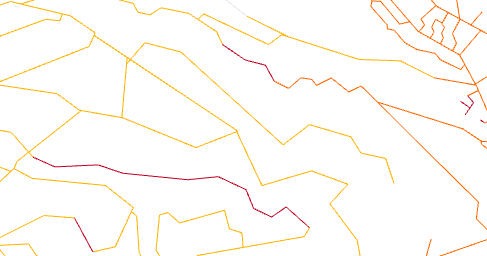
\includegraphics[width=\linewidth]{zuerich_street_error_cropped.png}
        \end{mdframed}
        \caption{Floating streets in the street network of Zurich}
        \label{fig:zuerich_error}
    \end{subfigure}
    \par\medskip
    \begin{subfigure}[b]{0.8\textwidth}
        \begin{mdframed}[style=mdthight]
            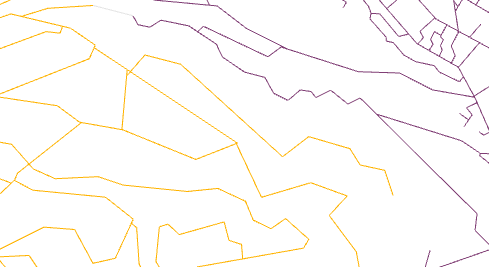
\includegraphics[width=\linewidth]{zuerich_street_fixed_cropped.png}
        \end{mdframed}
        \caption{Normalised street network of Zurich}
        \label{fig:zuerich_fixed}
    \end{subfigure}
    \caption{Street network of Zurich without (\ref{fig:zuerich_error}) and with (\ref{fig:zuerich_fixed}) normalisation}
\end{figure}

\section{Cluster colouring}
To visualize the clustering of a street network in this thesis, clusters are marked with different colours. This section describes the details of this cluster colouring.

The result of each clustering algorithm, which was implemented in this thesis, represents a cluster as set of vertices. Each of these vertices is a junction in the street network. The visualisation only draws streets but not the junctions, as the intersection of streets are intuitively seen as junctions. To colour the different clusters the following approach was taken:

\begin{itemize}
    \item Streets which connect two vertices that are part of the same cluster are coloured with that clusters colour.
    \item Streets which connect vertices of two distinct clusters are coloured grey.
\end{itemize}

There are papers which discuss how colours can be transformed to a perceptually uniform space, where the computation of $n$ colours with maximal distances (for the human eye) is possible \cite{colors:2006}.

In this thesis a more concise approach was taken: The papers of R. M. Boynton \cite{boynton:1989} and K. L. Kelly \cite{kelly:1965} define 11, respectively 22 colours, which are easy to distinguish by human eye. Those colours are displayed in figure \ref{fig:colours}.

Depending on the number of clusters one or the other of those colour sets (without black and white) were used. The colours were already sorted in a way that ensures the extraction of the first $n$ elements returns colours with maximal distance. If more than 20 clusters had to be coloured, the colours of Kelly were used multiple times.

\begin{figure}
    \centering
    \begin{subfigure}[b]{\textwidth}
        \begin{mdframed}[style=mdthight]
            
\includegraphics[width=\linewidth]{boynton_colours.png}
        \end{mdframed}
        \caption{Boynton colours}
        \label{fig:boynton_colours}
    \end{subfigure}
    \par\medskip
    \begin{subfigure}[b]{\textwidth}
        \begin{mdframed}[style=mdthight]
            
\includegraphics[width=\linewidth]{kelly_colours.png}
        \end{mdframed}
        \caption{Kelly colours}
        \label{fig:kelly_colurs}
    \end{subfigure}
    \caption{Colour palette of Boynton (\ref{fig:boynton_colours}) and Kelly (\ref{fig:kelly_colurs})}
    \label{fig:colours}
\end{figure}
